% !TEX root = ../main.tex

\section{Methodology}
\label{sec:method}

In this work, we sought to offer a high-level overview of Blockahin technology.
To accomplish this, we took the standard academic approach of surveying the available literature.
During this process, it became clear that the majority of work exploring Blockchain's capabilities and use cases comes from industry.\footnote{Here, we define industry as corporations, small and medium business, startups, and consortia.}

Materials produced by industry are sufficiently different from academic literature to make them difficult to use as sources in a traditional literature review.
In particular, there are three main concerns when reviewing materials that originated from industry:

\begin{enumerate}
	\item \textbf{Lack of precise terminology and discussion.}
	In our review of materials from industry, we found that the same concepts were often described using divergent and imprecise terminology, leading to muddled descriptions of capabilities and use cases.
	Additionally, while there is a fair bit of factually inaccurate information in materials from industry (e.g., several documents claimed cryptographic signatures provide confidentiality), in several cases we clearly observed that the underlying idea being described was accurate but was phrased in such a way as to make it seem incorrect under cursory examination.
	In this regard, materials from industry represent a trove of useful information obscured by imprecise terminology and discussion.
	
	\item \textbf{Inclusion of hype.}
	Much of the material from industry includes visionary statements (i.e., hype) regarding how Blockchain technology will change technology and the world.
	This hype is a mixture of realistic applications that can be built on top of Blockchain systems (e.g., anonymous payments~\cite{chaum1988untraceable}) and ideals that far transcend any technical solution (e.g., removing the need for governments).
	Unfortunately, unlike what one would expect in academic literature, the materials from industry often intermingle hype with technical details. This at least partially explains why some in academia are quick to dismiss sources from industry.
	
	\item \textbf{Researcher bias.}	
	Researcher bias is an obvious problem in any literature review---regardless of whether the source is academia or industry---and one that is often not explicitly addressed in systemization papers.
	The potential for bias is even stronger when reviewing materials from industry as academia's inherent caution when considering work from industry along with the two issues described above (i.e., lack of precise terminology, hype) make it easy to dismiss out of hand materials from industry.
	Additionally, being aware of the academic pedigree of Blockchain technology can make it easy to overlook the interesting use cases enabled by the composition of existing primitives.
	
\end{enumerate}

For all three of these reasons, it is tempting to exclude industry materials from a review of the literature on Blockchain technology.
However, we instead chose to look for a research methodology that would allow us to address these issues and still extract the underlying information discussed by industry.
Ultimately, we settled on using a well established research method---\emph{grounded theory}~\cite{glaser1965constant,strauss1990basics,corbin1990grounded} (also known as the constant comparative method).

Grounded theory is used to analyze qualitative data sources (e.g., user stories, interviews) and extract the underlying data and processes described across the myriad of gathered sources.\footnote{Grounded theory identifies data and processes that are supported across the body of sources and is not a method for creating a fine-grained breakdown of an individual document.}
In particular, grounded theory is designed to help researchers identify data and processes within qualitative data sources generated by humans and filled with imprecise terminology and descriptions.
Additionally, grounded theory limits the impact of researcher bias, ensuring that the data and processes are derived from the data and not from the researcher's preconceived notions of what the data says.
Grounded theory explicitly addresses the first and third problems we identified for evaluating materials from industry, and our hope was that it would also be able to separate the hype from the underlying data and processing; a hope which we believe was satisfied based on our results.

The idea of using grounded theory for literature review is not new~\cite{wolfswinkel2013using,yang2012descriptive} and this method has been used in thousands of studies examining qualitative data.\footnote{As evidence of its wide use, the top-cited paper describing grounded theory has 62,951 citations as of writing.}
%TODO: This needs to be anonymized when submitted.
For these reasons and based on our own experience with the method~\cite{ruoti2017weighing} we were confident this method would allow us to successfully accomplish our research goals.

In the remainder of this section we first describe how we gathered industry materials for our grounded theory analysis.
Next, we describe the grounded theory process in some detail, as it may be unfamiliar to readers in this field.
Lastly, we describe an academic literature review we conducted to enhance the results of our grounded theory analysis.

\subsection{Industry Material Gathering}
Beginning in the summer of 2016 we began to gather documents published in regards to Blockchain technology.
This included both materials from industry and academia, though this section will focus on only the former.
We gathered materials using a variety of methods:

\begin{itemize}
	\item Following RSS feeds that track news and publications related to Blockchain technology (e.g., CoinDesk\footnote{\url{https://coindesk.com}}).
	\item Downloaded materials published by Blockchain consortiums (e.g., Hyperledger\footnote{\url{https://www.hyperledger.org/}}, Decentralized Identity Framework\footnote{\url{http://identity.foundation/}}) and their members (e.g., IBM, Microsoft, Gem).
	\item Using Google to explore what was being said about Blockchain technology by major accounting firms, banks, and tech companies.
	\item Browsing new articles and blog posts related to Blockchain technology. This included articles which gave lists of interesting Blockchain papers.
	\item Reviewing submissions to the ONC Blockchain in Health Care Competition.\footnote{\url{https://www.healthit.gov/topic/grants-contracts/announcing-blockchain-challenge}}.
\end{itemize}

When reviewing these materials, we would also follow references and include those documents if we believe they were relevant.
In total, we collected 132 document.
The documents we gathered generally fell into one of three categories.

\begin{enumerate}
	\item \textbf{High-Level Overviews.} These were often prepared by investment firms and gave high level overviews of Blockchain technology. They would also reference various efforts at using Blockchain in practice.
	\item \textbf{System White Papers.} These papers would describe how Blockchain technology was used in a specific system, or more frequently a system proposal.
	\item \textbf{Blockchain Commentaries.} These were largely shorter documents that would discuss a specific facet of Blockchain technology in greater depth than we saw in other documents.
\end{enumerate}

\subsection{Grounded Theory Data Analysis}
After collecting our initial set of 104 documents, we analyzed them using grounded theory.
This methodology splits analysis of the documents into four stages: open coding, axial coding, selective coding, and theory generation.
Throughout the analysis of the documents we kept detailed research notes that outlined our thoughts as we reviewed and analyzed the literature.
Additionally, we conducted intensive discussion between the various researchers to ensure that we were correctly understanding and evaluating the source material.
As is often the case in grounded theory, these notes and discussion were every bit as important, if not more so, than the concepts, categories, and theories we generated.

\subsubsection{Stage 1---Open Coding}
In this first stage, documents were assigned to one of four reviewers.
Each reviewer would read the document, assign codes to words and sentences in the document.
These codes were generated using a mixture of open coding (assigning a code that summarizes the document's statement) and in situ coding (using the document's own words as the code).
To ensure that we were assigning the correct codes, we paid careful attention to the context of each statement.

In particular, reviewers made sure to code the following four concepts found in documents:
\begin{enumerate}
	\item \textbf{Properties.} What are the building blocks for Blockchain technology? What capabilities does it provide?
	\item \textbf{Challenges.} What challenges must be addressed when building systems using Blockchain technology?
	\item \textbf{Limitations.} What inherent limitations are their when using Blockchain technology?
	\item \textbf{Use cases.} What use cases are suitable for Blockchain technology?
\end{enumerate}

At this stage of the grounded theory process, reviewers were instructed to avoid evaluating the validity of the coded concepts.
Instead, every attempt was to made to include all possible codes, helping to ensure that our results were grounded in the data and not reviewers' biases.

The reviewers continued reviewing documents until each felt that the last 3--5 documents they had read had no concepts that had not already been brought up by previous documents.
This is a commonly accepted stopping criteria in grounded theory and is indicative that all core (i.e., not truly one-off) ideas have been discovered.
In total, this stage resulted in the creation of 641 codes.

\subsubsection{Stage 2---Axial Coding}
In the second stage, our research team used the constant comparative method to group codes into concepts.
Specifically, we collapsed distinct codes referring to the same topic (e.g., one was an open code, the other in situ) into a single code, reducing the original set of 641 codes to a more manageable 68 codes.
As needed, we referred back to the original documents to ensure that our understanding of the code was fresh, and that we were assigning it to the appropriate concept.
Also, at this stage we continued to avoid evaluating the validity of concepts, ensuring that the ideas of the reviewed documents were fully reflected in the codes.

\subsection{Interlude---Additional Open Coding}
After completing axial coding, one reviewer coded (i.e., open coding) another 28 documents.
These documents were all blog posts, representing the most up-to-date thinking on Blockchain technology.
In this process, no new codes were discovered, indicating that our process had produced concepts that thoroughly describe Blockchain technology.

\subsubsection{Stage 3---Selective Coding}
In the third stage, two researchers transfered all of the concepts onto sticky-notes.
They then drew connecting lines between the concepts, describing how the concepts related to one another.
Based on these interconnections, concepts were divided into five different categories:

\begin{enumerate}
	\item \textbf{Primitives.} These are the primitives that are used to enabled Blockchain technology. Unlike properties, they have no useful by themselves, but only when combined with other primitives to achieve specific properties. Examples include on-chain tokens, authenticated data-structures, and zero-knowledge proofs.
	
	\item \textbf{Technological properties.} Technological properties are the core building blocks and features of Blockchain technology. Examples include decentralized governance, append-only ledgers, and data replication.
	
	\item \textbf{Normative properties.} Normative properties differ from technological properties in that they are not technical, but rather represent properties that people hope to achieve through the use of Blockchain technology. Critically, these properties cannot be achieved through reliance on the technical properties alone, but require the system built on top of Blockchain technology be designed to accomplish these goals. Examples include censorship resistance, ease-of-entry for miners, low cost to participate.
	In general, normative properties roughly correlate to the hype attached to Blockchain technology.

	\item \textbf{Capabilities.} Capabilities are high-level features provided by Blockchain technology. Examples include on-chain asset provenance, anonymity, and resilience.
	
	\item \textbf{Use cases.} Use cases are the areas where the properties and capabilities of Blockchain technology would be useful in building systems. Examples include cryptocurrencies, supply chain management, and identity management.
\end{enumerate}

While we divide the concepts into five categories, the individual concepts between these categories were highly connected to each other.
Images of these category graphs can be found in Figure~\ref{fig:grounded-theory-main}~and~\ref{fig:grounded-theory-apps} .

\begin{figure*}
	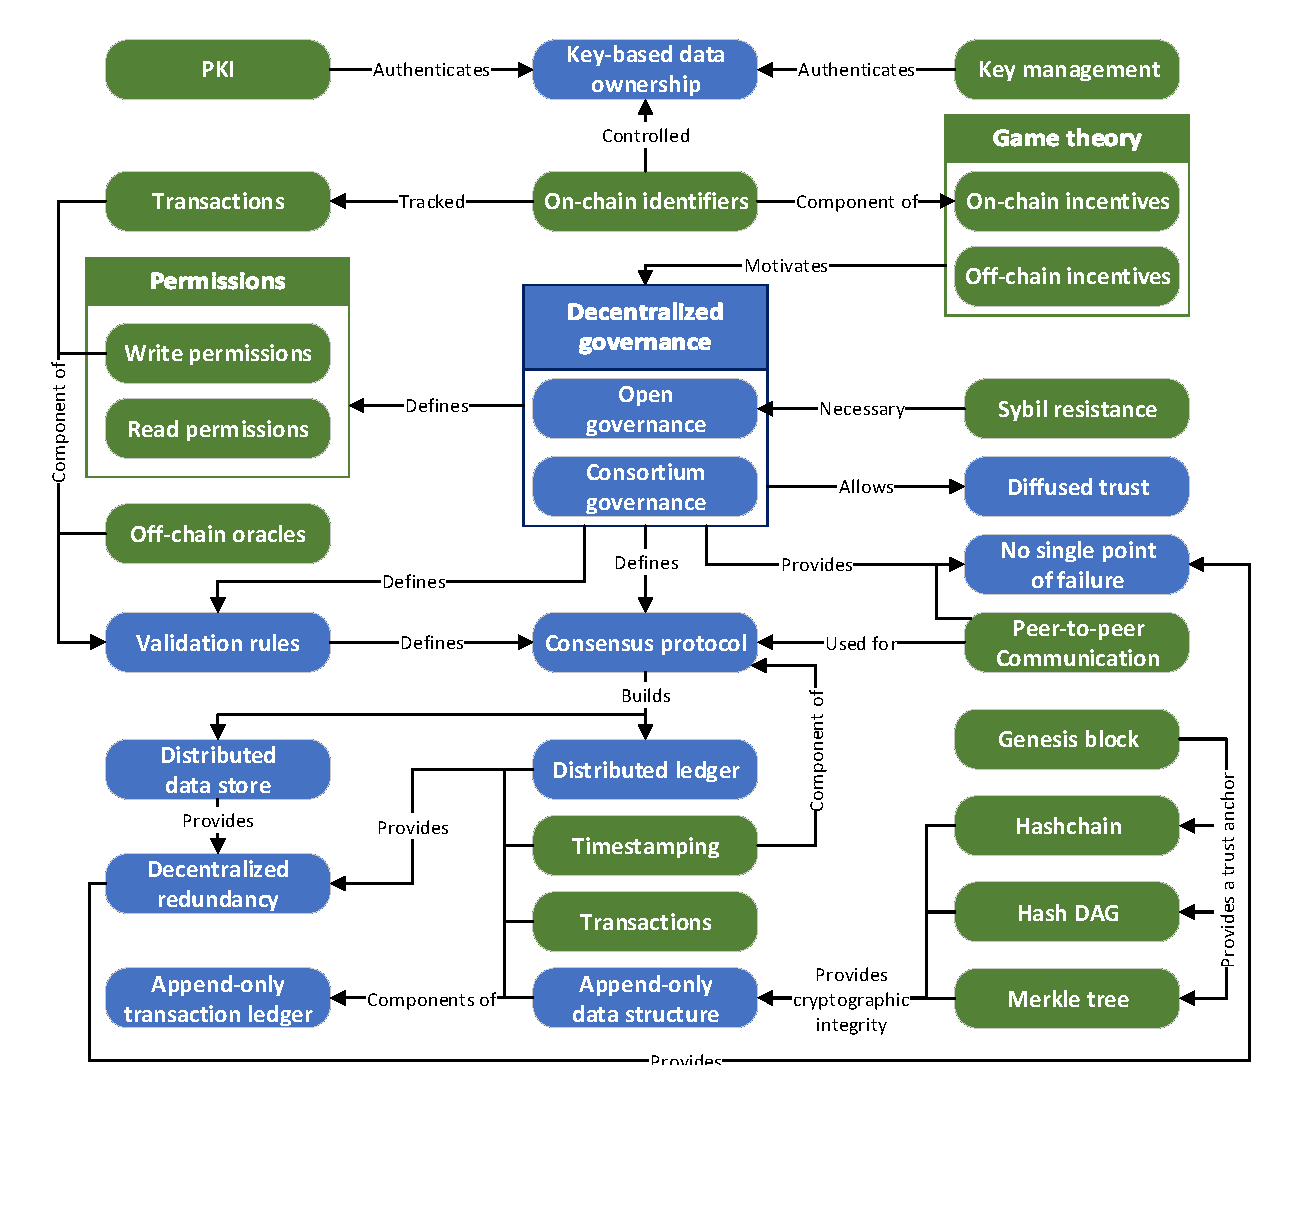
\includegraphics[width=\textwidth]{figures/grounded-theory-main}
	\caption{Category Map for Blockchain Technology.}
	\label{fig:grounded-theory-main}
\end{figure*}

\begin{figure*}
	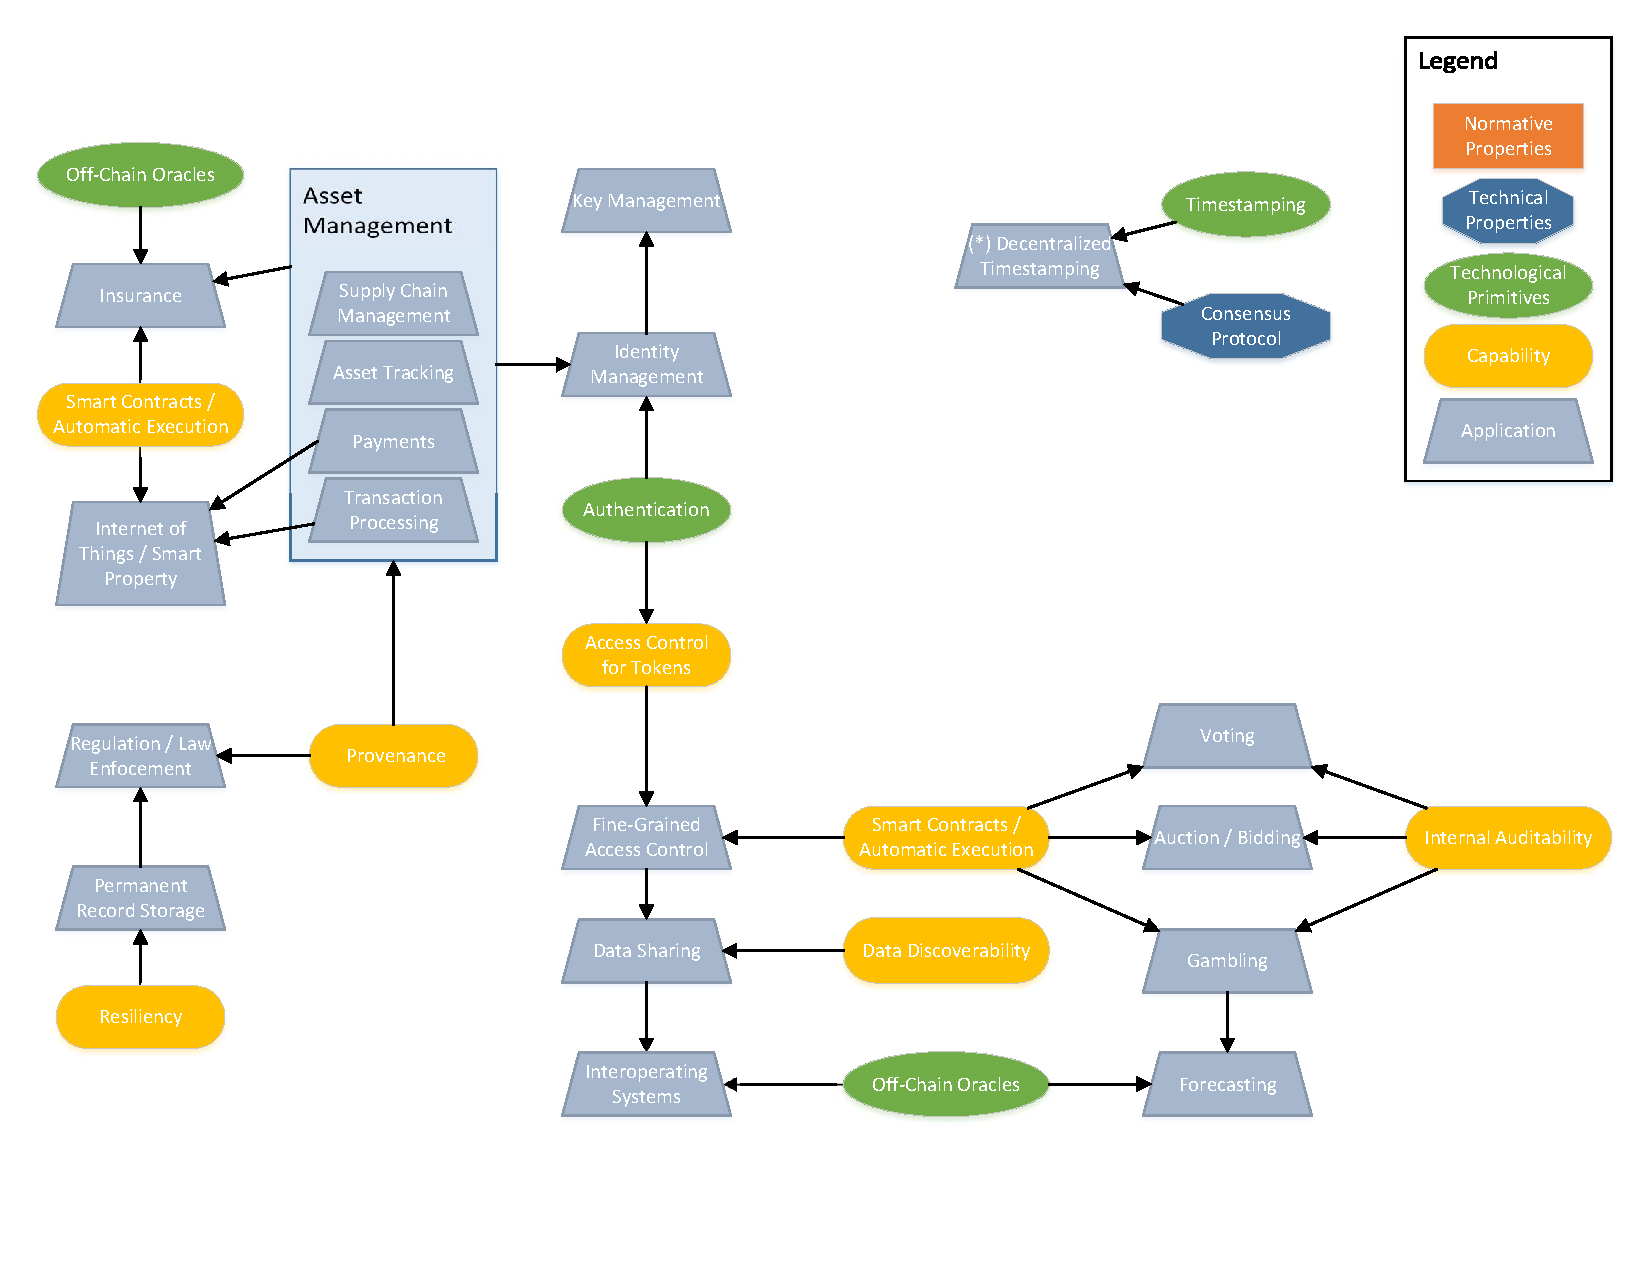
\includegraphics[width=\textwidth]{figures/grounded-theory-apps}
	\caption{Use Case Map for Blockchain Technology.}
	\label{fig:grounded-theory-apps}
\end{figure*}

At this stage of the research, we allowed researcher expertise to begin influencing the results.
First, by its very nature drawing connections between concepts is subjective.
As much as possible, we attempted to identify text in the underlying documents that supported our connections, but in several cases we created connections that were not explicitly mentioned in the text.
Second, a handful of primitives were added that we determined were necessary to build some of the technological properties, but had not been discussed in the documents.
Third, we identified several misconceptions that either shared no connections with the rest of the concepts or were obviously false (e.g., cryptographic signatures do not provide confidentiality).
In each of these three cases, our research notes kept track of what was explicitly supported by the analyzed data and what was the result of researcher interpretation.

\subsubsection{Stage 4---Theory Generation}
In the fourth and final stage, we used the categories, their connections, and our results to derive several theories (i.e., research results from our analysis) regarding Blockchain.
First, we derived a concrete set of properties and capabilities describing precisely what Blockchain technology is, and what it isn't.
Second, we were able to produce a clean split between Blokchain technology's technological primitives and its normative properties (i.e., hype).
Third, we identified criteria that help determine whether a given problem can benefit from the use of Blockchain technology.

\subsubsection{Limitations}
Due to the nature of grounded theory, our analysis of the data represents one view on that data.
Different researchers coding the same data may have focused on different aspects leading to differences in categories, connections, and the theories they focused on.
To address this limitation, we will make the documents we reviewed and our coding of those documents public.

\subsection{Academic Literature Review}
As part of the grounded theory analysis, the data revealed several open research challenges related to Blockchain technology.
In regards to these challenges, we conducted a review of academic literature to identify what research has already been done and what the academic community thinks of these challenges.
These challenges, along with the relevant paper references, are discussed in Section~\ref{sec:challenges}.